\documentclass[aspectratio=169,11pt]{beamer}

\usepackage[T1]{fontenc}
\usepackage[brazilian]{babel}
\usepackage{booktabs}
\usepackage{tabularx}
\graphicspath{{../../assets/}{figuras/}}
\makeatletter
\IfFileExists{beamerthemeEMASC.sty}{}{\def\input@path{{../modelo/}}}
\makeatother
\usetheme{EMASC}

\setlength{\parskip}{0.35em}
\setlength{\tabcolsep}{6pt}
\renewcommand{\arraystretch}{1.08}
\lstset{style=EMASC,language=Python}
\hypersetup{colorlinks=true,urlcolor=emascPurple,linkcolor=emascPurple,pdfencoding=auto}
\urlstyle{same}
\renewcommand*{\HyperDestNameFilter}[1]{ciencia-dados.#1}

\title{Introdução à Ciência de Dados}
\institute{Liga Acadêmica Matemática \& Empresa}
\date{EMASC 2026}

\begin{document}
\EMASCtitlepage{Introdução à\\Ciência de Dados}

\begin{frame}[t]{Roteiro}
\begin{enumerate}
  \item \hyperlink{cd-problema}{\textbf{Problema e bibliotecas}}
  \item \hyperlink{cd-numpy}{\textbf{NumPy}}
  \item \hyperlink{cd-pandas}{\textbf{pandas}}
  \item \hyperlink{cd-preparacao}{\textbf{Preparação dos dados}}
  \item \hyperlink{cd-analise}{\textbf{Análise e visualização}}
  \item \hyperlink{cd-resultado}{\textbf{Interpretação e resultado}}
\end{enumerate}
\end{frame}

\section{Problema e bibliotecas}

\begin{frame}[t,label=cd-problema]{O que é Ciência de Dados?}
Ciência de Dados combina programação, Matemática e Estatística para analisar dados e apoiar decisões.
\begin{EMASCnote}
\textbf{Problema de estudo:} uma equipe acadêmica acompanha as notas de três cursos. Em quais há notas pendentes? Como se distribuem as notas disponíveis?
\end{EMASCnote}
\smallskip
\textbf{Base de dados:} 18 registros fictícios. Alguns exemplos:
\begin{tabularx}{\linewidth}{@{}lXrrr@{}}
\toprule
\texttt{id} & \texttt{curso} & \texttt{horas\_estudo} & \texttt{frequencia} & \texttt{nota} \\
\midrule
1 & Matematica & 2,0 & 0,70 & 5,9 \\
6 & Matematica & 3,5 & 0,80 & \\
\bottomrule
\end{tabularx}
\smallskip

\small
O ID identifica o estudante. A frequência é a proporção de aulas frequentadas (0,70 = 70\%). O campo vazio indica nota ainda não registrada neste exemplo.
\end{frame}

\begin{frame}[t]{Etapas de uma análise}
\begin{enumerate}
  \item \textbf{Entender o problema:} definir a pergunta que os dados deverão ajudar a responder.
  \item \textbf{Obter os dados:} reunir as informações necessárias à análise.
  \item \textbf{Preparar os dados:} verificar tipos, valores ausentes e inconsistências.
  \item \textbf{Explorar os dados:} calcular medidas estatísticas e construir gráficos.
  \item \textbf{Interpretar os resultados:} identificar padrões e reconhecer limitações.
  \item \textbf{Propor uma ação:} utilizar os resultados para justificar uma decisão e acompanhar sua aplicação.
\end{enumerate}
\end{frame}

\begin{frame}[fragile,t]{Bibliotecas de Python}
Uma biblioteca reúne funções e estruturas prontas para uso.

\begin{tabularx}{\linewidth}{@{}lX@{}}
\toprule
\textbf{Biblioteca} & \textbf{Aplicação} \\
\midrule
NumPy & Operações com vetores, matrizes e cálculos numéricos. \\
pandas & Leitura, manipulação e análise de dados tabulares. \\
Matplotlib & Construção de gráficos e visualização de dados. \\
\bottomrule
\end{tabularx}
\EMASCcodelabel{Importação}
\begin{lstlisting}
import numpy as np
import pandas as pd
import matplotlib.pyplot as plt
\end{lstlisting}
Os nomes \texttt{np}, \texttt{pd} e \texttt{plt} são abreviações das bibliotecas.
\end{frame}

\section{NumPy}

\begin{frame}[fragile,t,label=cd-numpy]{1. Arrays}
Um \textit{array} do NumPy armazena elementos do mesmo tipo. Diferentemente de uma lista, permite realizar cálculos numéricos diretamente com seus elementos.
\EMASCcodelabel{Exemplo prático}
\begin{lstlisting}
notas = np.array([5.9, 6.7, 7.5, 8.2, 9.1])
print(notas)
print(notas.dtype)   # Tipo dos elementos
print(notas.ndim)    # Numero de dimensoes
print(notas.shape)   # (5,), cinco elementos
print(notas[0])      # Primeiro elemento
print(notas[1:4])    # Elementos de indices 1 a 3
\end{lstlisting}
\begin{EMASCnote}
O índice começa em zero. O índice final de uma fatia não entra no resultado.
\end{EMASCnote}
\end{frame}

\begin{frame}[fragile,t]{1.1. Matrizes}
Um array com duas dimensões pode representar uma matriz. O atributo \texttt{shape} indica o número de linhas e colunas.
\EMASCcodelabel{Horas de estudo e notas de dois estudantes}
\begin{lstlisting}
matriz = np.array([[2.0, 5.9],
                   [3.0, 6.7]])

print(matriz.shape)    # (2, 2)
print(matriz[0, 1])    # 5.9
print(matriz[:, 0])    # Primeira coluna
print(matriz[1, :])    # Segunda linha
\end{lstlisting}
\begin{EMASCnote}
Em uma matriz, \texttt{matriz[i, j]} acessa o elemento da linha \texttt{i} e coluna \texttt{j}.
\end{EMASCnote}
\end{frame}

\begin{frame}[fragile,t]{1.2. Criação de arrays}
\begin{tabularx}{\linewidth}{@{}lX@{}}
\toprule
\textbf{Função} & \textbf{Descrição} \\
\midrule
\texttt{np.zeros(n)} & Array com $n$ zeros. \\
\texttt{np.ones(n)} & Array com $n$ uns. \\
\texttt{np.arange(inicio, fim, passo)} & Passo fixo, sem incluir o fim. \\
\texttt{np.linspace(inicio, fim, n)} & $n$ valores equidistantes, inclui o fim. \\
\bottomrule
\end{tabularx}
\EMASCcodelabel{Exemplos complementares para consulta}
\begin{lstlisting}
print(np.zeros(3))          # [0. 0. 0.]
print(np.ones(3))           # [1. 1. 1.]
print(np.arange(0, 10, 2))  # [0 2 4 6 8]
print(np.linspace(0, 10, 6)) # [0. 2. 4. 6. 8. 10.]
\end{lstlisting}
\end{frame}

\begin{frame}[fragile,t]{1.3. Operações vetorizadas}
Arrays de mesmo formato operam elemento a elemento. Exemplo: horas de estudo dos mesmos três estudantes em duas semanas.
\EMASCcodelabel{Exemplo prático}
\begin{lstlisting}
semana1 = [2, 3, 4]
semana2 = [3, 4, 5]
print(semana1 + semana2)  # [2, 3, 4, 3, 4, 5]
total = np.array(semana1) + np.array(semana2)
print(total)           # [5 7 9], horas de estudo
print(total / 2)       # Media semanal por estudante
print(notas >= 7)      # Comparacao elemento a elemento
\end{lstlisting}
\begin{EMASCnote}
Em listas, \texttt{+} concatena os elementos. Em arrays, soma elemento a elemento. A comparação retorna valores booleanos.
\end{EMASCnote}
\end{frame}

\begin{frame}[fragile,t]{1.4. Medidas estatísticas com NumPy}
As funções do NumPy permitem calcular as medidas estudadas na parte de Estatística.
\EMASCcodelabel{Exemplo prático}
\begin{lstlisting}
print("Média:", np.mean(notas))
print("Mediana:", np.median(notas))
print("Mínimo:", np.min(notas))
print("Máximo:", np.max(notas))
print("Desvio populacional:", np.std(notas, ddof=0))
print("Desvio amostral:", np.std(notas, ddof=1))
\end{lstlisting}
\begin{EMASCnote}
Na variância, \texttt{ddof=0} usa $n$ para descrever a população. Utilize \texttt{ddof=1} (divisor $n-1$) quando a amostra serve para estimar a variância populacional.
\end{EMASCnote}
\end{frame}

\section{pandas}

\begin{frame}[fragile,t,label=cd-pandas]{2. Series e DataFrame}
\begin{itemize}
  \item \textbf{Series:} sequência de valores, cada um com seu índice.
  \item \textbf{DataFrame:} tabela com linhas e colunas que podem ter tipos diferentes.
\end{itemize}
\begin{columns}[T,onlytextwidth]
\begin{column}{0.54\textwidth}
\EMASCcodelabel{Exemplo prático}
\begin{lstlisting}
serie = pd.Series([5.9, 6.7, 7.5])
exemplo = pd.DataFrame({
    "id": [1, 2, 3],
    "nota": [5.9, 6.7, 7.5]
})
print(serie)
print(exemplo)
\end{lstlisting}
\end{column}
\begin{column}{0.42\textwidth}
\EMASCcodelabel{DataFrame}
\begin{tabular}{rrr}
\toprule
\textbf{Índice} & \textbf{id} & \textbf{nota} \\
\midrule
0 & 1 & 5.9 \\
1 & 2 & 6.7 \\
2 & 3 & 7.5 \\
\bottomrule
\end{tabular}
\smallskip

A coluna \texttt{nota} com seus índices é uma Series.
\end{column}
\end{columns}
\end{frame}

\begin{frame}[fragile,t]{2.1. Leitura de uma base de dados}
CSV é um arquivo de texto com dados separados por um delimitador, geralmente vírgula.
\EMASCcodelabel{Sintaxe}
\texttt{pd.read\_csv("notas.csv")}
\EMASCcodelabel{Leitura do arquivo de notas}
\begin{lstlisting}
df = pd.read_csv(fonte)
print(df.head())
\end{lstlisting}
\begin{EMASCnote}
A função aceita um caminho local ou uma URL. A variável \texttt{fonte} é definida na célula de configuração do notebook.
\end{EMASCnote}
\medskip
Para arquivos separados por ponto e vírgula, utilize \texttt{sep=";"}.
\end{frame}

\begin{frame}[fragile,t]{2.2. Inspeção dos dados}
Antes de realizar cálculos, é importante conhecer o formato da tabela e o significado das colunas.
\EMASCcodelabel{Exemplo prático}
\begin{lstlisting}
print("Primeiras linhas:\n", df.head())
print("Ultimas linhas:\n", df.tail())
print("Linhas e colunas:", df.shape)
print("Colunas:", df.columns)
df.info()   # Tipos e quantidade de valores presentes
print(df[["horas_estudo", "frequencia", "nota"]].describe())
\end{lstlisting}
\begin{EMASCnote}
\texttt{shape} retorna \texttt{(18, 5)}. \texttt{describe()} resume as variáveis numéricas; o ID foi excluído por ser um identificador.
\end{EMASCnote}
\end{frame}

\begin{frame}[fragile,t]{2.3. Seleção de linhas e colunas}
\texttt{loc} seleciona por rótulos. \texttt{iloc} seleciona por posições inteiras, iniciadas em zero.
\EMASCcodelabel{Exemplo prático}
\begin{lstlisting}
print(df["nota"])                      # Uma Series
print(df[["curso", "nota"]])           # Um DataFrame
print(df.loc[0:2, ["id", "nota"]])     # Rotulos
print(df.iloc[0:3, [0, 4]])            # Posicoes
\end{lstlisting}
\begin{EMASCnote}
Os dois últimos comandos retornam as mesmas linhas e colunas. No \texttt{loc}, inclui-se o rótulo final; no \texttt{iloc}, exclui-se a posição final.
\end{EMASCnote}
\end{frame}

\begin{frame}[fragile,t]{2.4. Filtros e ordenação}
Filtros selecionam linhas que satisfazem condições. \texttt{isna()} identifica valores ausentes.
\EMASCcodelabel{Exemplo prático}
\begin{lstlisting}
print(df[df["curso"] == "Matematica"])
alto = (df["nota"] >= 7) & (df["frequencia"] >= 0.8)
print(df[alto])
atencao = (df["nota"] < 7) | (df["nota"].isna())
print(df[atencao])
print(df.sort_values("nota", ascending=False).head())
\end{lstlisting}
\begin{EMASCnote}
Use \texttt{\&}, \texttt{|} e \texttt{\textasciitilde} no lugar de \texttt{and}, \texttt{or} e \texttt{not} para comparar linha a linha. \texttt{ascending=False} ordena do maior para o menor.
\end{EMASCnote}
\end{frame}

\section{Preparação dos dados}

\begin{frame}[fragile,t,label=cd-preparacao]{3. Qualidade dos dados}
Após conferir os tipos das colunas, verificam-se registros repetidos, ausentes (\texttt{NaN}) e valores fora dos limites esperados.
\EMASCcodelabel{Exemplo prático}
\begin{lstlisting}
print("Duplicatas:", df.duplicated().sum())
print("IDs repetidos:", df["id"].duplicated().sum())
print("Ausentes:\n", df.isna().sum())
fora = df["nota"].notna() & ~df["nota"].between(0, 10)
print("Notas fora de 0 a 10:\n", df[fora])
\end{lstlisting}
\begin{EMASCnote}
\texttt{sum()} conta os valores \texttt{True} como 1. Há duas notas ausentes; a tabela vazia indica que nenhuma nota registrada está fora de 0 a 10.
\end{EMASCnote}
\end{frame}

\begin{frame}[fragile,t]{3.1. Tratamento de valores ausentes}
Existem diferentes formas de tratar valores ausentes. A escolha depende do significado desses valores e do objetivo da análise.
\EMASCcodelabel{Exemplo prático}
\begin{lstlisting}
pendentes = df[df["nota"].isna()]
print(pendentes[["id", "curso"]])

df_com_notas = df.dropna(subset=["nota"]).copy()
print("Linhas e colunas:", df_com_notas.shape)
\end{lstlisting}
\begin{EMASCnote}
Uma nota ausente não significa nota zero. Os 18 registros ficam em \texttt{df}; \texttt{dropna()} mantém apenas os 16 com nota na cópia.
\end{EMASCnote}
\small
\texttt{fillna(valor)} é outra possibilidade, quando a substituição puder ser justificada. Neste problema, substituir notas inventaria informações.
\end{frame}

\begin{frame}[fragile,t]{3.2. Criação de colunas}
Novas colunas podem ser calculadas ou obtidas por meio de uma função. Vamos converter a frequência em porcentagem e classificar as notas.
\EMASCcodelabel{Exemplo prático}
\begin{lstlisting}
df_com_notas["frequencia_pct"] = df_com_notas["frequencia"] * 100
def classificar(nota):
    if nota >= 7:
        return "Nota >= 7"
    return "Nota < 7"
df_com_notas["situacao"] = df_com_notas["nota"].apply(classificar)
print(df_com_notas[["frequencia_pct", "nota", "situacao"]].head())
\end{lstlisting}
\begin{EMASCnote}
\texttt{apply()} aplica a função a cada nota. O limite 7 é didático, não uma regra oficial de aprovação.
\end{EMASCnote}
\end{frame}

\section{Análise e visualização}

\begin{frame}[fragile,t,label=cd-analise]{4. Agrupamento dos dados}
\texttt{groupby("curso")} separa a tabela por curso. Podemos calcular uma medida para cada grupo, ou várias com \texttt{agg()}.
\EMASCcodelabel{Notas disponíveis por curso}
\begin{lstlisting}
print(df_com_notas.groupby("curso")["nota"].median())
resumo = df_com_notas.groupby("curso")["nota"].agg(
    ["count", "mean", "median", "std", "min", "max"]
)
print(resumo.round(2))
print(df_com_notas.groupby("curso")["situacao"].value_counts())
\end{lstlisting}
\begin{EMASCnote}
\texttt{count} conta as notas disponíveis, \texttt{std} é o desvio padrão amostral e \texttt{value\_counts()} conta quantas notas há em cada categoria.
\end{EMASCnote}
\end{frame}

\begin{frame}[fragile,t]{4.1. Frequência relativa de notas ausentes}
Ao selecionar um registro ao acaso dentro de um curso, a probabilidade de sua nota estar ausente é:
\[
  P(\text{nota ausente}\mid\text{curso}) =
  \frac{\text{notas ausentes no curso}}{\text{registros no curso}}
\]
\EMASCcodelabel{Exemplo prático}
\begin{lstlisting}
cobertura = df.groupby("curso")["nota"].agg(["size", "count"])
cobertura["sem_nota"] = cobertura["size"] - cobertura["count"]
cobertura["pct_sem_nota"] = 100 * cobertura["sem_nota"] / cobertura["size"]
print(cobertura.round(2))
\end{lstlisting}
\begin{EMASCnote}
\texttt{size} conta todas as linhas e \texttt{count} ignora ausentes. Em Matemática, $1/6\approx 16{,}67\%$ (probabilidade condicional na base).
\end{EMASCnote}
\end{frame}

\begin{frame}[fragile,t]{5. Matplotlib / Gráfico de barras}
O gráfico de barras compara categorias: os cursos no eixo $x$ e o percentual de notas ausentes no eixo $y$.
\EMASCcodelabel{Percentual de notas ausentes por curso}
\begin{lstlisting}
plt.rcParams["font.size"] = 13   # Tamanho da fonte
plt.figure(figsize=(6, 4))       # Largura e altura
barras = plt.bar(cobertura.index, cobertura["pct_sem_nota"],
                 color="#358FD0")
plt.bar_label(barras, fmt="%.1f%%") # Valores nas barras
plt.title("Notas ausentes por curso")
plt.xlabel("Curso")
plt.ylabel("Notas ausentes (%)")
plt.ylim(0, 100)
plt.tight_layout()               # Ajusta o espaco
plt.show()                       # Exibe o grafico
\end{lstlisting}
\end{frame}

\begin{frame}[t]{5.1. Comparação dos cursos}
\begin{columns}[T,onlytextwidth]
\begin{column}{0.62\textwidth}
\centering
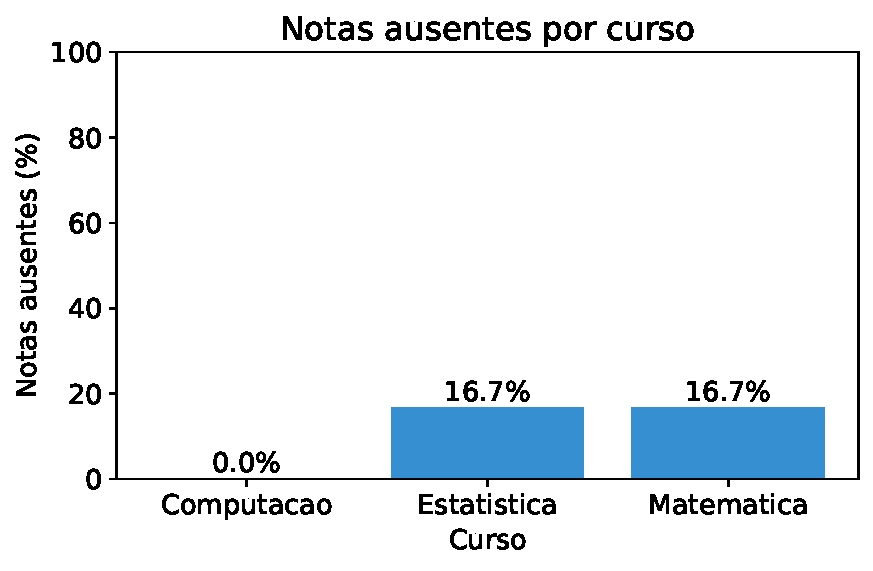
\includegraphics[width=\linewidth]{barras.pdf}
\end{column}
\begin{column}{0.35\textwidth}
\medskip
\textbf{Interpretação}
\begin{itemize}
  \item Matemática e Estatística: uma nota ausente em seis registros.
  \item Computação: todas as notas estão disponíveis.
\end{itemize}
\end{column}
\end{columns}
\end{frame}

\begin{frame}[fragile,t]{5.2. Histograma}
O histograma representa a distribuição de uma variável numérica. As barras mostram quantos valores pertencem a cada intervalo.
\EMASCcodelabel{Distribuição das notas disponíveis}
\begin{lstlisting}
plt.figure(figsize=(6, 4))
plt.hist(df_com_notas["nota"], bins=5, color="#358FD0", edgecolor="white")
plt.title("Distribuição das notas")
plt.xlabel("Nota")
plt.ylabel("Frequência absoluta")
plt.tight_layout()
plt.show()
\end{lstlisting}
\begin{EMASCnote}
\texttt{bins=5} define cinco intervalos de mesma largura entre a menor e a maior nota. As alturas são as contagens por intervalo.
\end{EMASCnote}
\end{frame}

\begin{frame}[t]{5.3. Distribuição das notas}
\begin{columns}[T,onlytextwidth]
\begin{column}{0.62\textwidth}
\centering
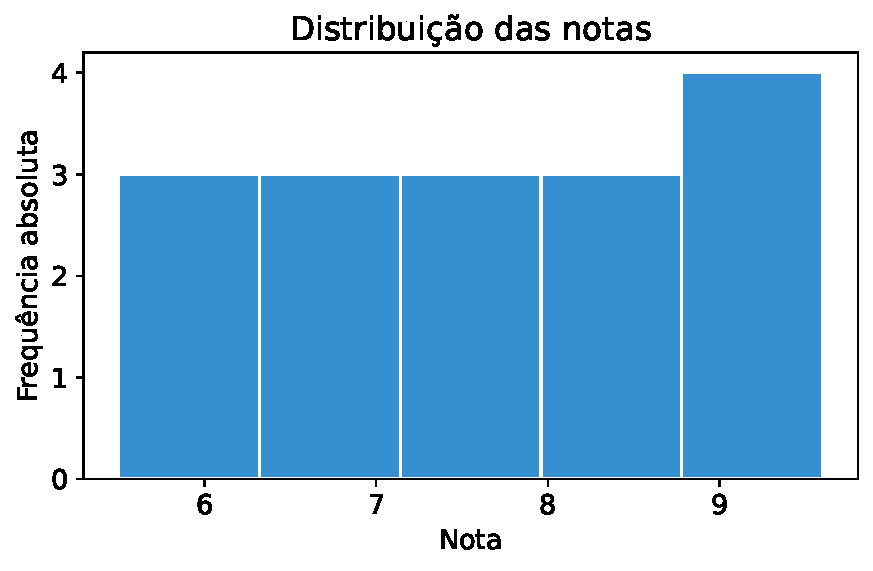
\includegraphics[width=\linewidth]{histograma.pdf}
\end{column}
\begin{column}{0.35\textwidth}
\medskip
\textbf{Interpretação}
\begin{itemize}
  \item As notas disponíveis variam de 5,5 a 9,6.
  \item Os quatro primeiros intervalos contêm três notas cada, e o último contém quatro.
\end{itemize}
\end{column}
\end{columns}
\end{frame}

\begin{frame}[fragile,t]{5.4. Gráfico de dispersão}
O gráfico de dispersão mostra a relação entre duas variáveis numéricas.
\EMASCcodelabel{Relação entre frequência e nota}
\begin{lstlisting}
plt.figure(figsize=(6, 4))
for curso, grupo in df_com_notas.groupby("curso"):
    plt.scatter(grupo["frequencia_pct"], grupo["nota"], label=curso)
plt.title("Frequência e nota")
plt.xlabel("Frequência (%)")
plt.ylabel("Nota")
plt.legend()
plt.tight_layout()
plt.show()
\end{lstlisting}
\begin{EMASCnote}
O laço separa os pontos por curso. \texttt{label} nomeia o grupo e \texttt{legend()} exibe a legenda.
\end{EMASCnote}
\end{frame}

\begin{frame}[t]{5.5. Relação entre frequência e nota}
\begin{columns}[T,onlytextwidth]
\begin{column}{0.62\textwidth}
\centering
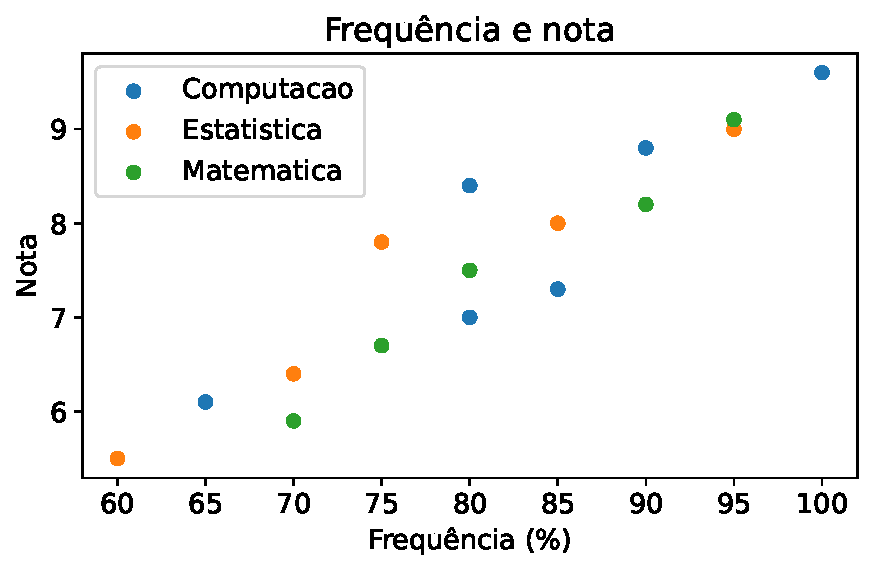
\includegraphics[width=\linewidth]{dispersao.pdf}
\end{column}
\begin{column}{0.35\textwidth}
\medskip
\textbf{Interpretação}
\begin{itemize}
  \item Nesta base, notas maiores tendem a acompanhar frequências mais altas.
  \item Essa associação, por si só, não demonstra uma relação de causa e efeito.
\end{itemize}
\end{column}
\end{columns}
\end{frame}

\section{Interpretação e resultado}

\begin{frame}[t,label=cd-resultado]{6. Interpretação e proposta de ação}
\begin{tabularx}{\linewidth}{@{}lXrrr@{}}
\toprule
\textbf{Curso} & \textbf{Disponíveis} & \textbf{Mediana} & \textbf{Desvio padrão} & \textbf{Ausentes} \\
\midrule
Computação & 6 & 7,85 & 1,29 & 0,0\% \\
Estatística & 5 & 7,80 & 1,38 & 16,7\% \\
Matemática & 5 & 7,50 & 1,25 & 16,7\% \\
\bottomrule
\end{tabularx}
\smallskip

\textbf{Análise:} medianas e desvios padrão próximos entre os cursos.

\textbf{Ação proposta:} conferir as duas notas pendentes com os responsáveis.

\textbf{Avaliação:} buscar 0\% de notas ausentes e repetir a análise.

\begin{EMASCnote}
A base é pequena e fictícia. As medidas descrevem as notas disponíveis, não a qualidade dos cursos.
\end{EMASCnote}
\end{frame}

\begin{frame}[fragile,t]{6.1. Junção de tabelas}
O método \texttt{merge()} combina tabelas a partir de uma coluna em comum. Vamos juntar as medidas das notas ao percentual de notas ausentes pelo curso.
\EMASCcodelabel{Exemplo prático}
\begin{lstlisting}
ausencias = cobertura[["pct_sem_nota"]].reset_index()
resultado = pd.merge(resumo.reset_index(), ausencias, on="curso")
print(resultado.round(2))
\end{lstlisting}
\begin{EMASCnote}
\texttt{reset\_index()} transforma o índice dos cursos em uma coluna. \texttt{on="curso"} indica a coluna usada para relacionar as tabelas.
\end{EMASCnote}
\end{frame}

\begin{frame}[fragile,t]{6.2. Exportação dos resultados}
A tabela final pode ser exportada para utilização em relatórios ou novas análises.
\EMASCcodelabel{Exemplo prático}
\begin{lstlisting}
resultado.round(2).to_csv(
    "resumo_por_curso.csv",
    index=False
)
print("Arquivo resumo_por_curso.csv gerado.")
\end{lstlisting}
\begin{EMASCnote}
\texttt{to\_csv()} grava a tabela em um arquivo CSV. \texttt{index=False} impede que o índice numérico seja gravado como uma coluna adicional.
\end{EMASCnote}
\end{frame}

\begin{frame}[t,label=referencias-ciencia-dados]{Referências}
\begin{itemize}
  \item NUMPY. \textit{NumPy documentation}. Disponível em: \url{https://numpy.org/doc/}.
  \item PANDAS. \textit{pandas documentation}. Disponível em: \url{https://pandas.pydata.org/docs/}.
  \item MATPLOTLIB. \textit{Matplotlib documentation}. Disponível em: \url{https://matplotlib.org/stable/}.
  \item LAME. \textit{Guia de Apoio: Fundamentos de Python, Estatística e Bibliotecas}. EMASC 2026.
\end{itemize}
\end{frame}

\end{document}
